\documentclass[18pt]{beamer}
\usepackage[utf8]{inputenc} % for the umlauts
\usepackage{subfigure}

\beamertemplatenavigationsymbolsempty
%% SLIDE FORMAT

% use 'beamerthemekit' for standard 4:3 ratio
% for widescreen slides (16:9), use 'beamerthemekitwide'

\usepackage{templates/beamerthemekit}
% \usepackage{templates/beamerthemekitwide}

\setcounter{tocdepth}{1}

%% TITLE PICTURE

% if a custom picture is to be used on the title page, copy it into the 'logos'
% directory, in the line below, replace 'mypicture' with the 
% filename (without extension) and uncomment the following line
% (picture proportions: 63 : 20 for standard, 169 : 40 for wide
% *.eps format if you use latex+dvips+ps2pdf, 
% *.jpg/*.png/*.pdf if you use pdflatex)

%\titleimage{mypicture}

%% TikZ INTEGRATION

% use these packages for PCM symbols and UML classes
% \usepackage{templates/tikzkit}
% \usepackage{templates/tikzuml}

% the presentation starts here

\usepackage{mathabx}
\usepackage{picture}
\usepackage[absolute,overlay]{textpos}
%\usepackage[texcoord,grid,gridunit=mm,gridcolor=red, subgridcolor=green]{eso-pic}
\setbeamercovered{invisible}
\setbeamertemplate{caption}{\raggedright\insertcaption\par}

\title[SWT1]{Softwaretechnik 1 - 6. Tutorium}
\subtitle{Tutorium 03}
\author{Felix Bachmann}
\date{24.07.2017}

\institute{KIT - Institut für Programmstrukturen und Datenorganisation (IPD)}

% Bibliography

\usepackage[citestyle=authoryear,bibstyle=numeric,hyperref,backend=biber]{biblatex}
\addbibresource{templates/example.bib}
\bibhang1em

\begin{document}
	
% change the following line to "ngerman" for German style date and logos
\selectlanguage{ngerman}
\setcounter{tocdepth}{2}
	
%title page
\begin{frame}
\titlepage
\end{frame}

\begin{frame}
\tableofcontents
\end{frame}


\section{Orga}
	\subsection{Allgemeines}
	\begin{frame}
		\frametitle{Allgemeines}
		%TODO ?
	\end{frame}

	\subsection{Feedback}
	\begin{frame}
		\frametitle{6. Übungsblatt Statistik}
		%TODO statistics 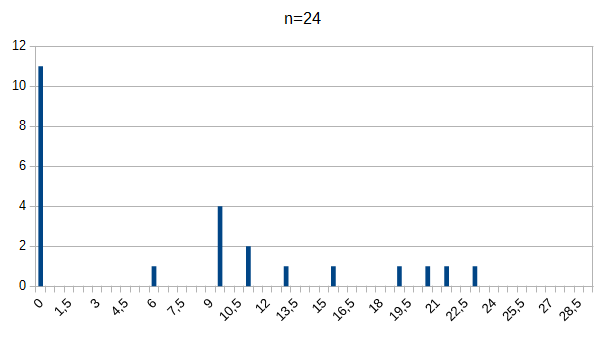
\includegraphics[scale=0.7]{./pics/tut5/statistics-ub5-2.png}
		%TODO avg \linebreak \centering $\diameter$ von 26+4
	\end{frame}

	\begin{frame}
		\frametitle{Häufige Fehler}
		\begin{block}{Allgemein}
			\begin{itemize}
				\item %TODO ?
			\end{itemize}
		\end{block}
	\end{frame}

	\begin{frame}
		\frametitle{Häufige Fehler}
		\begin{block}{Aufgabe 1 (Kontrollfluss-orientiertes Testen): $\diameter$ von 5+1} %TODO avg
			\begin{itemize}
				\pause 
				\item %TODO
			\end{itemize}
		\end{block}
	\end{frame}

	\begin{frame}
		\frametitle{Häufige Fehler}
		\begin{block}{Aufgabe 2 (Codeinspektion): $\diameter$ von 4} %TODO avg
			\begin{itemize}
				\pause 
				\item %TODO 
			\end{itemize}
		\end{block}
		\pause 
		\begin{block}{Aufgabe 3 (Parallelisierung von Geometrify): $\diameter$  von 5} %TODO avg
			\begin{itemize}
				\pause
				\item %TODO 
			\end{itemize}
		\end{block}
	\end{frame}

	\begin{frame}
		\frametitle{Häufige Fehler}
		\begin{block}{Aufgabe 4 (Alternative Parallelisierungsvarianten): $\diameter$ von 6+3} %TODO avg
			\begin{itemize}
				\pause
				\item %TODO
			\end{itemize}
		\end{block}
		\pause
		\begin{block}{Aufgabe 5 (Parallelisierungswettbewerb): $\diameter$ von 6} %TODO avg
			\begin{itemize}
				\pause
				\item %TODO
			\end{itemize}
		\end{block}
	\end{frame}
		
\section{Testen}
	\subsection{KFO}
	\begin{frame}
		\frametitle{Kontrollflussorientiertes Testverfahren (KFO)}
		\begin{itemize}
			\item Ziel: "'sinnvolle"' Testfälle finden
		\end{itemize}
		Vorgehen:
		\begin{enumerate}
			\item gegeben: zu testender Code \pause
			\item Code $\implies$ Zwischensprache
			\begin{itemize}
				\item Sprünge umwandeln
				\item Grundblöcke finden
				\item Grundblöcke prüfen
			\end{itemize}
			\pause
			\item Zwischensprache $\implies$ Kontrollflussgraph \pause
			\item am Kontrollflussgraphen Testfälle finden: \pause
			\begin{itemize}
				\item Anweisungsüberdeckung
				\item Zweigüberdeckung 
				\item Pfadüberdeckung
			\end{itemize}
		\end{enumerate}
	\end{frame}

	\begin{frame}
		\frametitle{KFO: Code nach Zwischensprache}
		\begin{itemize}
			\item Sprünge umwandeln
		\end{itemize}
		\centering 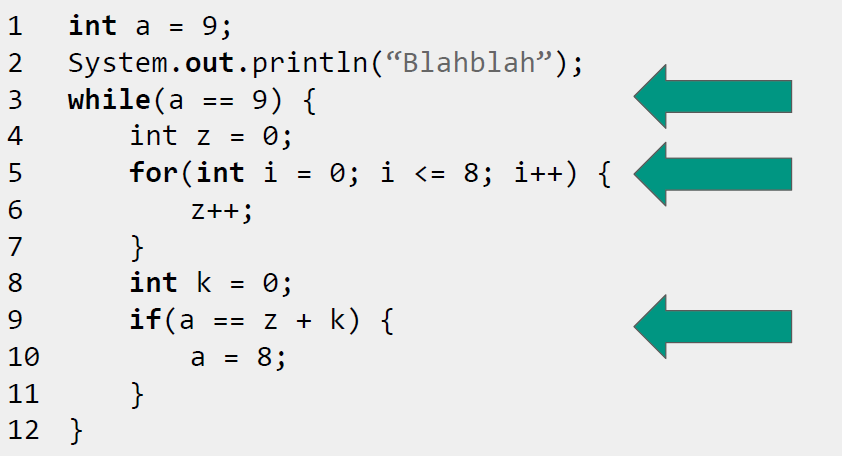
\includegraphics[scale=0.34]{./pics/tut5/code.png}
	\end{frame}

	\begin{frame}
		\frametitle{KFO: Code nach Zwischensprache}
		\begin{itemize}
			\item Sprünge umwandeln
		\end{itemize}
		\centering 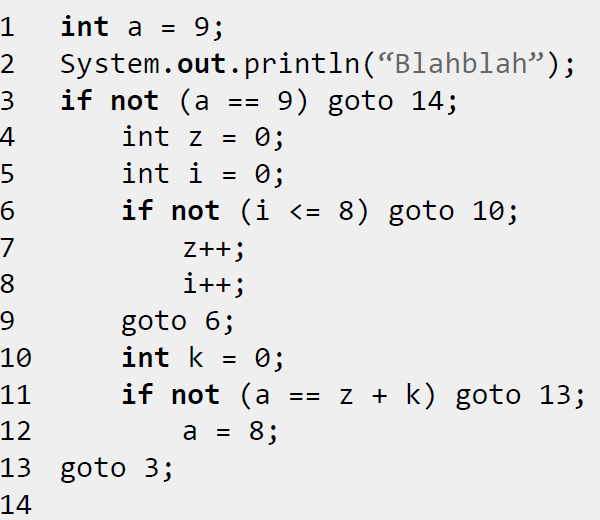
\includegraphics[scale=0.34]{./pics/tut5/code-jumps.png}
	\end{frame}

	\begin{frame}
		\frametitle{KFO: Code nach Zwischensprache}
		\begin{itemize}
			\item Grundblöcke finden (Code bis goto ist ein Grundblock)
		\end{itemize}
		\centering 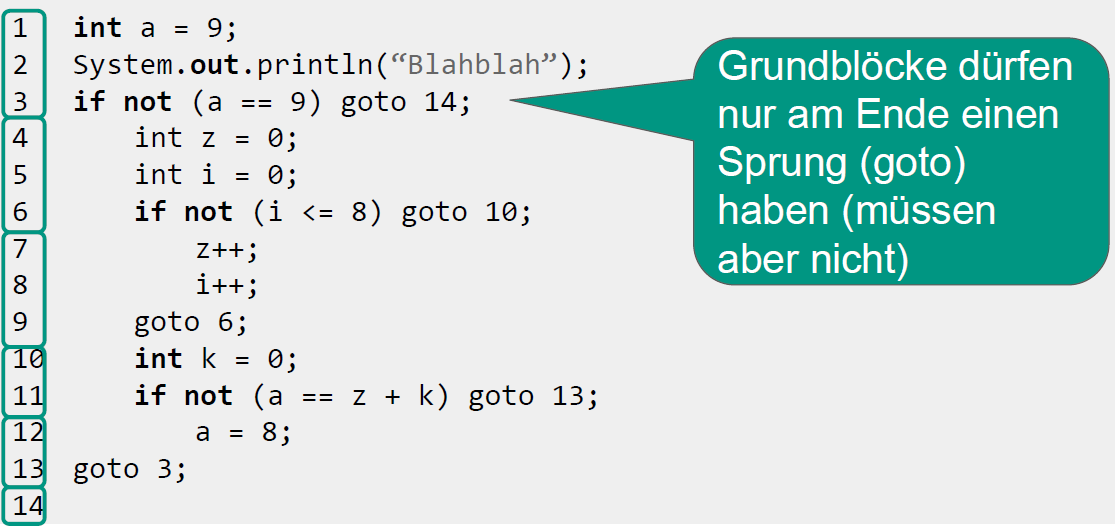
\includegraphics[scale=0.34]{./pics/tut5/first-blocks.png}
	\end{frame}

	\begin{frame}
		\frametitle{KFO: Code nach Zwischensprache}
		\begin{itemize}
			\item 	Grundblöcke prüfen (goto dürfen nur an Anfang eines Grundblocks verweisen)
		\end{itemize}
			\centering 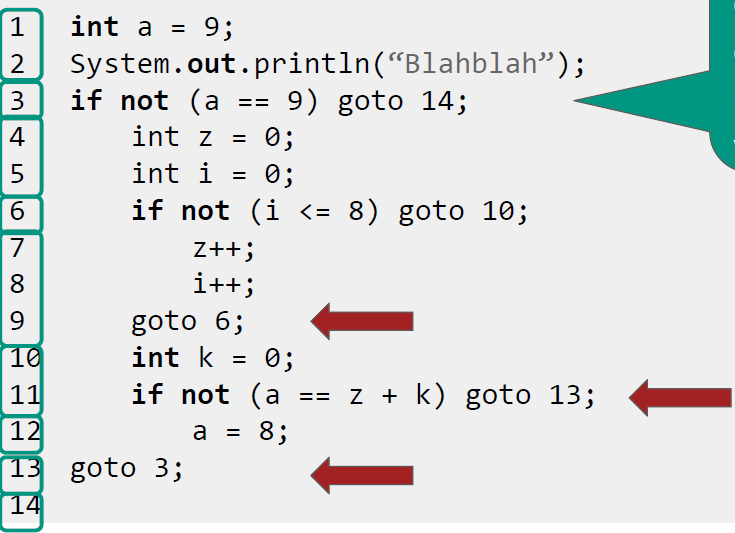
\includegraphics[scale=0.34]{./pics/tut5/second-blocks.png}
	\end{frame}

	\begin{frame}
		\frametitle{KFO: Zwischensprache nach Kontrollflussgraph}
		\begin{itemize}
			\item Grundblöcke benennen
			\item Grundblöcke und Verzweigungen hinzeichnen
			\item Start- und Endzustand hinzufügen
		\end{itemize}
	\end{frame}

	\begin{frame}
		\frametitle{KFO: Zwischensprache nach Kontrollflussgraph}
		\centering 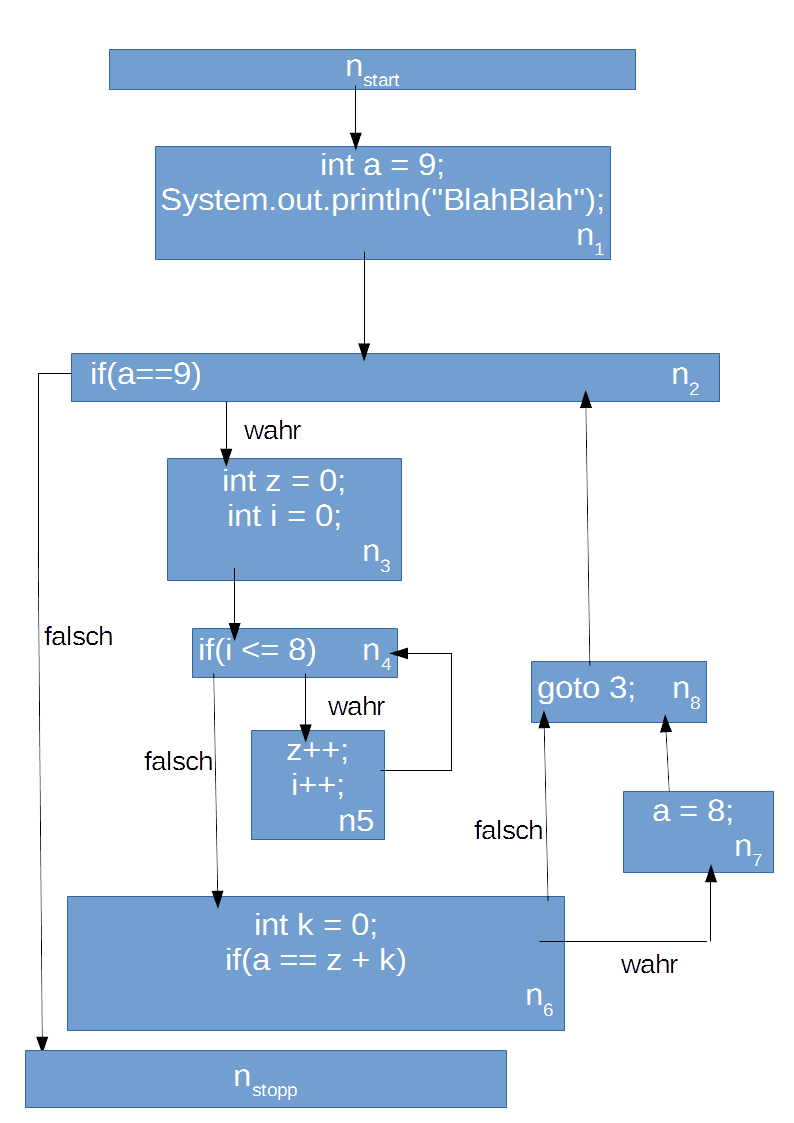
\includegraphics[scale=0.25]{./pics/tut5/test.png}
	\end{frame}

	\begin{frame}
		\frametitle{KFO: Zwischensprache nach Kontrollflussgraph}
		\begin{itemize}
			\item goto-Knoten kann man auch weglassen
		\end{itemize}
		\centering 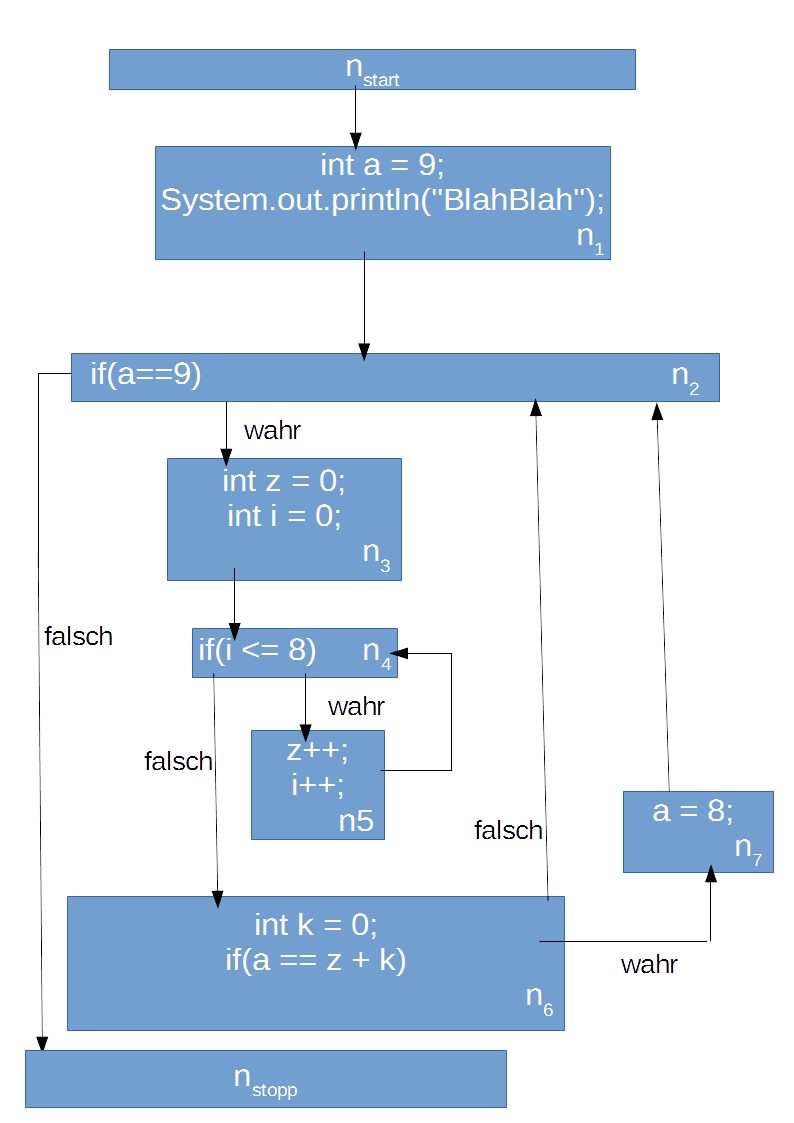
\includegraphics[scale=0.2]{./pics/tut5/test-without-goto.png}
	\end{frame}

	\begin{frame}
		\frametitle{KFO: Anweisungsüberdeckung}
		\begin{itemize}
			\item Pfade finden, sodass jeder Grundblock traversiert wird \pause
			\linebreak $\implies$ Entdeckung nicht erreichbarer Code-Abschnitte \pause
			\item aber: kein ausreichendes Testkriterium
		\end{itemize}
	\end{frame}

	\begin{frame}
		\frametitle{KFO: Anweisungsüberdeckung}
		\centering 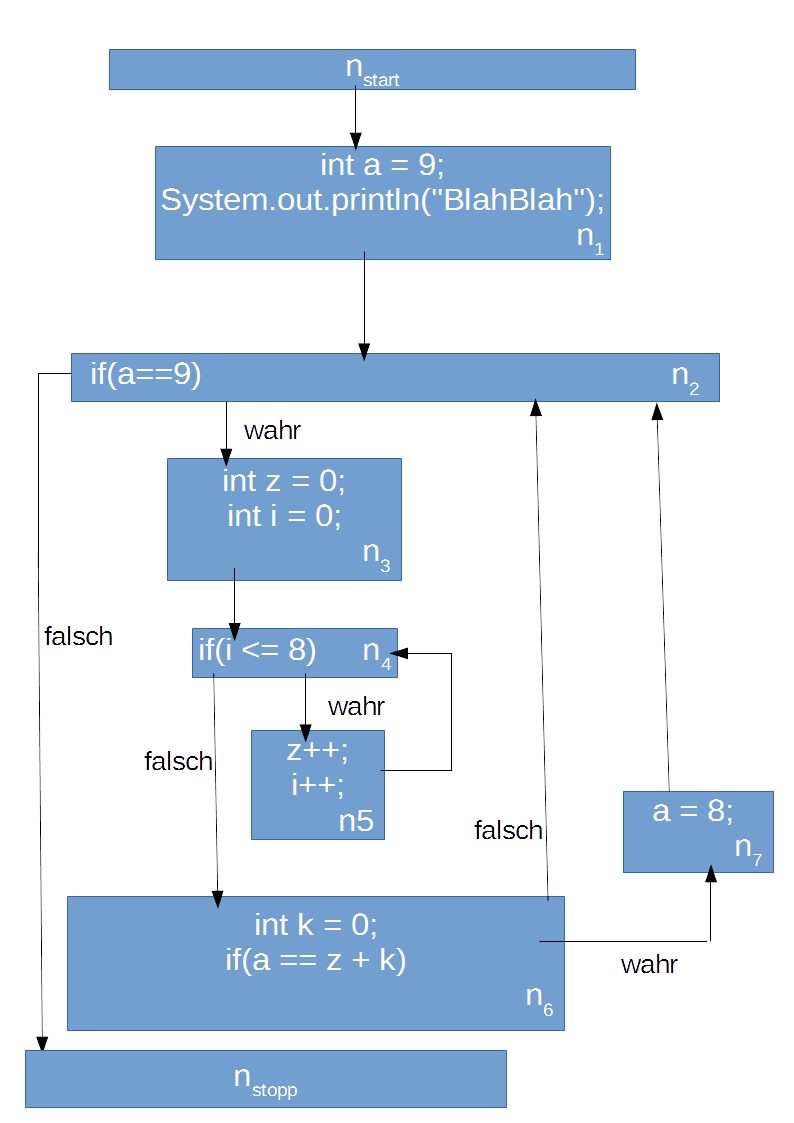
\includegraphics[scale=0.2]{./pics/tut5/test-without-goto.png}
		\begin{itemize}
			\item Pfad für Anweisungsüberdeckung? \pause ($n_{start}, n_1, n_2, n_3, n_4, n_5, n_4, n_6, n_7, n_2, n_{stopp}$) 
		\end{itemize}
	\end{frame}

	\begin{frame}
		\frametitle{KFO: Zweigüberdeckung}
		\begin{itemize}
			\item Pfade finden, sodass jeder Zweig (=Kante) traversiert wird \pause
			\linebreak $\implies$ Entdeckung nicht erreichbarer Kanten \pause
			\item aber: Schleifen werden nicht ausreichend getestet
		\end{itemize}
	\end{frame}

	\begin{frame}
		\frametitle{KFO: Zweigüberdeckung}
		\centering 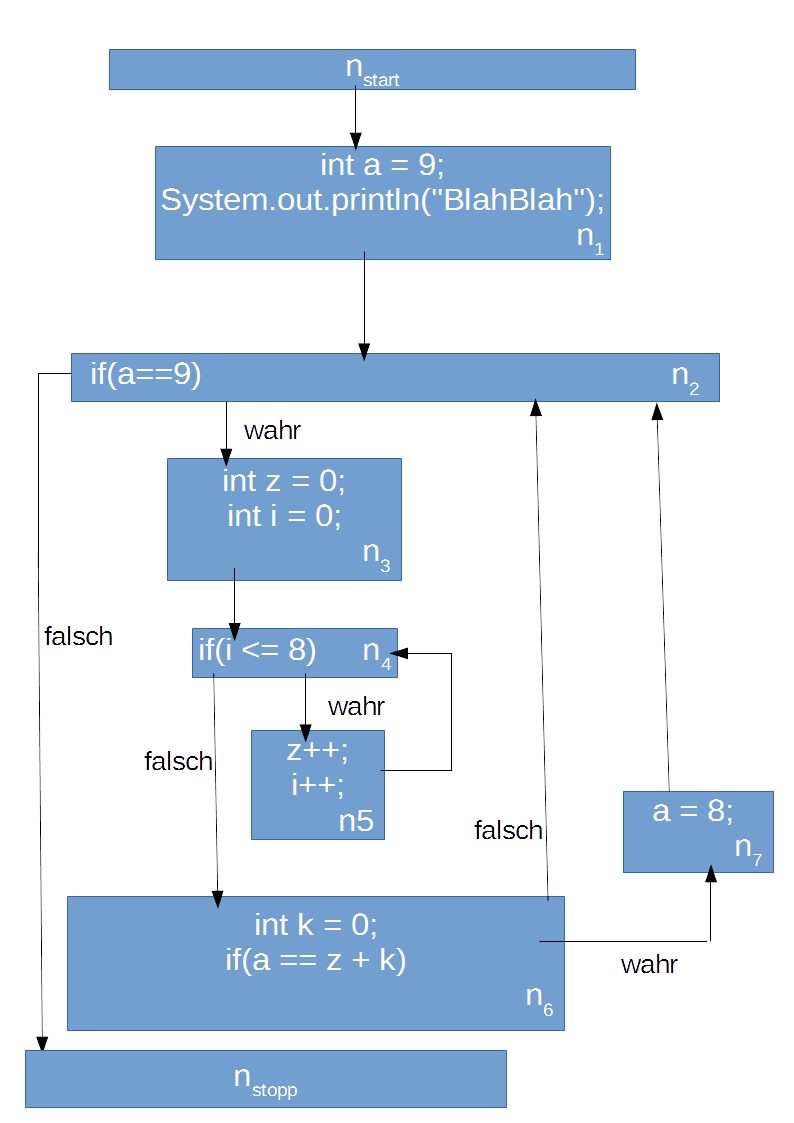
\includegraphics[scale=0.2]{./pics/tut5/test-without-goto.png}
		\begin{itemize}
			\item Pfad für Zweigüberdeckung? \pause ($n_{start}, n_1, n_2, n_3, n_4, n_5, n_4, n_6, n_2, n_3, n_4, n_5, n_4, n_6, n_7, n_2, n_{stopp}$) 
		\end{itemize}
	\end{frame}

	\begin{frame}
		\frametitle{KFO: Pfadüberdeckung}
		\begin{itemize}
			\item Finde \textbf{alle} vollständige, unterschiedlichen Pfade \pause
			\item vollständiger Pfad = Anfang bei $n_{start}$, Ende bei $n_{stopp}$ \pause
			\item nicht praktikabel, da 
			\begin{itemize}
				\item Schleifen die Anzahl der möglichen Pfade stark erhöhen \pause
				\item manche Pfade nicht ausführbar sind (sich gegenseitig ausschließende Bedingungen)
			\end{itemize}
		\end{itemize}
	\end{frame}

		
	\begin{frame}
		\frametitle{Klausuraufgabe SS11}
		\centering 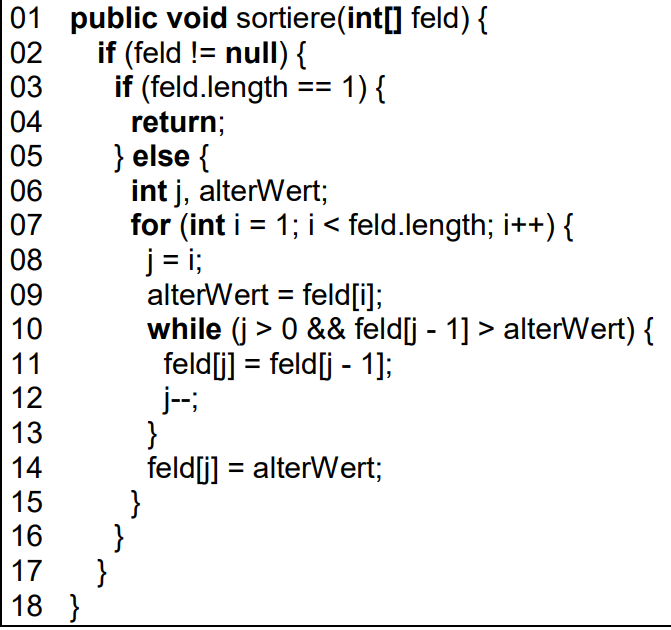
\includegraphics[scale=0.4]{./pics/tut5/exam-task-kfo.png}
		\linebreak
		Erstellen Sie den Kontrollflussgraphen und geben Sie einen Pfad an, der Anweisungsüberdeckung erzielt.
	\end{frame}

	\begin{frame}
		\frametitle{MuLö KFO}
		\centering 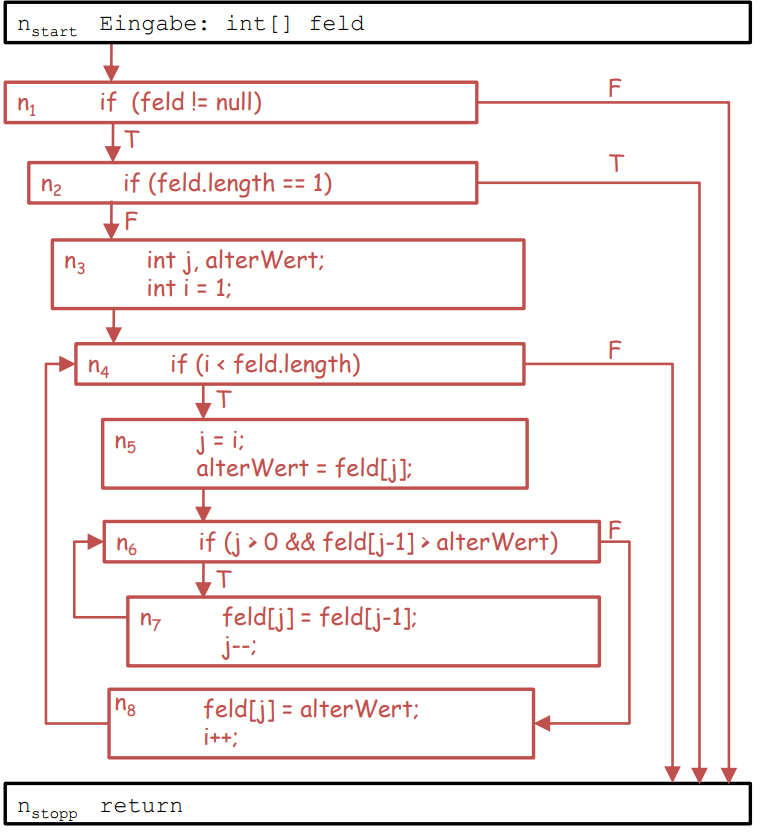
\includegraphics[scale=0.3]{./pics/tut5/exam-task-kfo-sol.png}
		\linebreak \pause
		Pfad: ($n_{start}, n_1, n_2, n_3, n_4, n_5, n_6, n_7, n_6, n_8, n_4, n_{stopp}$) 
	\end{frame}

\section{Wiederholung und Klausuraufgaben}

	\subsection{Planung \& Definition}
	\begin{frame}
		\frametitle{Disclaimer}
		\begin{large}
			\begin{itemize}
				\item Ich kenne die Klausur auch nicht! \pause
				\linebreak $\implies$ alles, was ich zum Inhalt der Klausur sage ist Spekulation
				\begin{itemize}
					\item basierend auf Altklausuren \pause
				\end{itemize}
				\item kein Anspruch auf Vollständigkeit der Wiederholung
			\end{itemize}
		\end{large}
	\end{frame}

	\begin{frame}
		\frametitle{Die typische SWT-Klausur}
		\begin{enumerate}
			\item Aufgabe 1: Wahr-/Falsch-Fragen (ein paar gesammelt auf \url{www.github.com/malluce/swt1-tut})
			 und Wissensfragen\pause
			\item meistens:
			\begin{itemize}
				\item 1-2 Aufgaben zu UML-Diagrammen \pause
				\item 1 Aufgabe zu Entwurfsmustern \pause
				\item 1 Aufgabe zu Parallelität \pause
				\item 1 Aufgabe zu Testen bzw. Qualitätssicherung \pause
				\item 1 Aufgabe Rest (z.B. Objektorientierung, Abbott, Prozessmodelle\dots) \pause
			\end{itemize}
		\end{enumerate}
		\begin{itemize}
			\item 1/3$\pm \epsilon$ der Punkte reichen zum Bestehen
		\end{itemize}
	\end{frame}

	\begin{frame}
		\frametitle{Planung \& Definition}
		\begin{itemize}
			\item Lastenheft, Pflichtenheft \pause
			\begin{itemize}
				\item Phasen zuordnen \pause
				\item Gliederung kennen \pause
				\item Beispiele geben \pause
			\end{itemize}
			\item UML-Diagramme \pause
			\begin{itemize}
				\item Klassendiagramm \pause
				\item Aktivitäts-, Sequenz-, Zustandsdiagramm \pause 
				\item Anwendungsfalldiagramm \pause
				\item Syntax kennen! \pause
				\item gegebenen Text in Diagramm umwandeln \pause
				\item bei Zustandsd.: Umwandeln hierarchisch $\Leftrightarrow$ nicht-hierarchisch
			\end{itemize}
		\end{itemize}
	\end{frame}

	%TODO exam task?

	\subsection{Entwurf}
	\begin{frame}
		\frametitle{Entwurf}
		\begin{itemize}
			\item Architekturstile \pause
			\item \textbf{Entwurfsmuster} \pause
			\begin{itemize}
				\item möglichst viele, bestenfalls alle kennen und verstehen \pause
				\item Kategorien kennen \pause
				\item Klassendiagramm hinzeichnen \pause
				\item aus Klassendiagrammen Entwurfsmuster erkennen \pause
				\item Code für einfache Muster (Singleton\dots) schreiben \pause
				\item Code-Schnipsel auf mögliche Verbesserung durch EM untersuchen
			\end{itemize}
		\end{itemize}
	\end{frame}

	%TODO exam task?
	
	\subsection{Implementierung}
	
	\subsection{Testen}
	
	\subsection{Abnahme, Einsatz \& Wartung}

\section{Ende}
	\begin{frame}
		\frametitle{Lernen}
		\begin{itemize}
			\item Klausuren rechnen $\land$ Folien anschauen \linebreak $>$ Klausuren rechnen XOR Folien anschauen
		\end{itemize}
	\end{frame}

	\begin{frame}
		\frametitle{Das war's dann wohl\dots}
		\centering
		\begin{huge}
			Viel Erfolg bei der Klausur und im weiteren Studium! :)
		\end{huge}
		\linebreak
		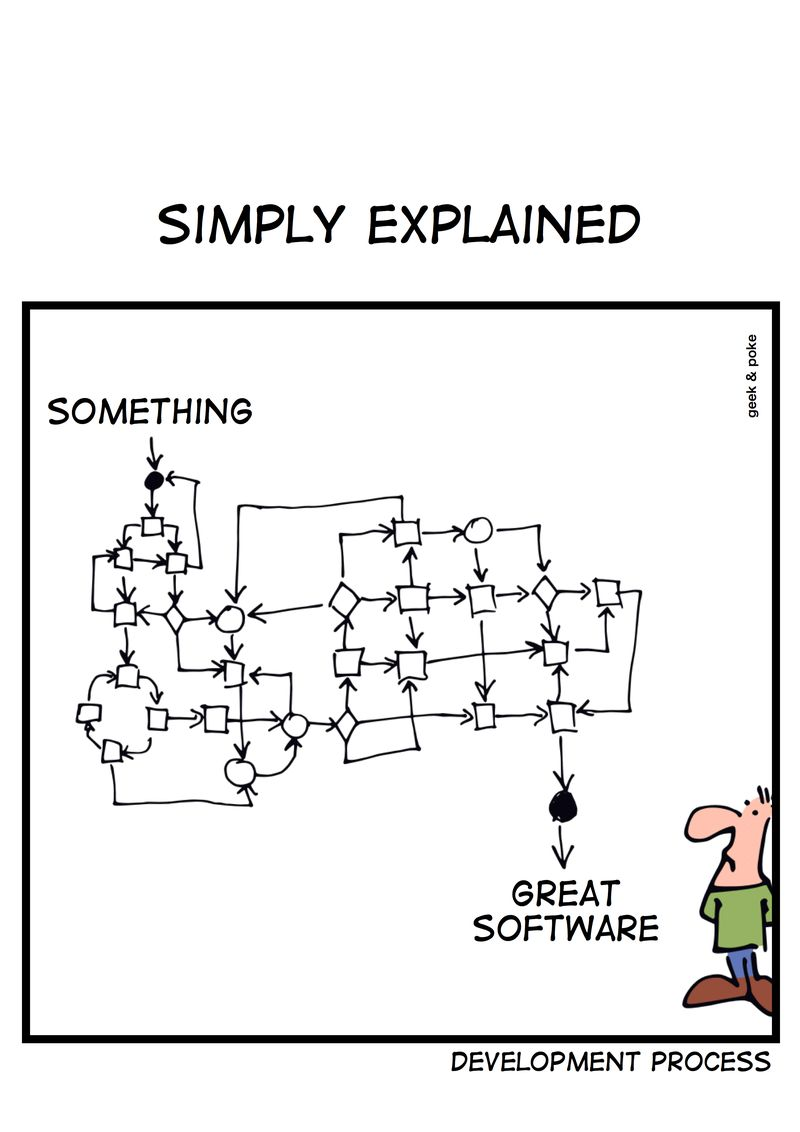
\includegraphics[scale=0.6]{./comics/geek_and_poke_development2.jpg}
	\end{frame}

\end{document}